\section{Signed boundary barriers and convergence of the full curve}
\label{sec:curves}

We now pass from the torus laws to the domains and exterior contours in
Theorem~\ref{thm:main}.  Theorem~\ref{thm:bulk-stability} compares finite
vectors of polygonal spin tests in the pure and perturbed tori.
Proposition~\ref{prop:strict-incidence} transfers colored crossings from
those tori to the target domain, after suitable boundary paths have been
revealed.  These crossings will place the target trace between two pure
comparison chords with the same limiting $\SLE_3$ law.

Identifying a trace does not determine its traversal order.  We use the
other output of Section~\ref{sec:comparison}, the fixed-buffer density
bound in Proposition~\ref{prop:interior-density}, to transfer the bulk
four-passage estimate to target interior events.  It rules out reverse
travel of positive diameter along the limiting chord and gives the
oriented curve metric~\eqref{eq:curve-metric}.  Thus density comparison
controls exceptional events; the colored-barrier argument identifies the
limiting law.

Fix a permitted $J,U$, and choose the perturbation interval small enough
for Theorem~\ref{thm:critical-trajectory}, Theorem~\ref{thm:bulk-stability},
and Proposition~\ref{prop:strict-incidence}.  No further reduction depending
on a domain will be made.  Throughout this section the perturbed model is
at $\beta_c(J,U,\lambda)$, and $\mu_{\lambda,N}$ denotes its torus spin
law.  The pure torus law is $\mu_{0,N}$.  Write
\[
 D_n=\delta_n D_{\Omega_n},\qquad
 \gamma_n=\delta_n\gamma(P_n).
\]
By Lemma~\ref{lem:contour-spin}, its spin law is the conditional law
$\nu_{\Omega_n,\beta_c,\lambda}^{\tau_n}$ with the actual exterior
configuration $\tau_n$ induced by $P_{o,n}$.  We keep $\gamma_n$ as the
prescribed resolution of $P_n$ and its two half-stubs.  Spin paths and
bulk passage tests use the fixed triangulation of
Section~\ref{sec:stability}.  In a bulk face, triangular interpolation
and the prescribed contour have the same connections and differ by
$O(\delta_n)$ with their traversal order preserved.

At the boundary one must distinguish the prescribed interface from the
zero set obtained by interpolating the entire exterior spin field.
Exterior-only disagreement edges can enter a boundary face and change
its full-plane connections.  We will instead redraw the target locally
beside the signed strips, using the geometric filling proved in
Lemma~\ref{lem:curves-local-barrier}.  This changes its drawing by
$O(\delta_n)$ and leaves the conditional spin law with exterior
$\tau_n$ intact.

\subsection{Fixed displaced domains and their boundary incidences}

Let $I_+$ and $I_-$ be the two open arcs of $\partial D$ carrying the plus
and minus exterior nearest neighbors.  There are only two choices.  It
suffices to treat a subsequence on which this choice is fixed.  Choose a
Jordan--Schoenflies homeomorphism $\Psi$ of the plane
\cite[Section~1 and Section~2(A), p.~860]{Cairns1951} such that
\[
 D=\Psi(\{\rho<1\}),\quad
 a=\Psi(1),\quad b=\Psi(-1),\quad
 I_+=\Psi(\{e^{i\theta}:0<\theta<\pi\}).
\]
Only the topology of these coordinates is used.  All spin tests will be
fixed polygonal tests in the original Euclidean coordinates.

We first construct a domain favoring minus, from which plus crossings
can be transferred to the target.  Move its plus boundary outward and
its minus boundary inward.  A minus corridor will screen the target's
minus arc, while a disjoint plus corridor will screen the comparison
domain's plus arc.  Conditioning a torus on both crossings then permits
the two strict-incidence comparisons.  The caps must extend beyond the
boundaries they screen, so that a common free component cannot go
around them.

For an explicit construction, take $0<h<\pi/30$, also small enough that
$3h<1/2$, and let $R_h$ be the continuous periodic
function which is $1+3h$ on $[4h,\pi-4h]$, is $1-3h$ outside
$(3h,\pi-3h)$, and is affine on the two remaining transition intervals.
The preliminary comparison domain is
\begin{equation}
 A_h^{\mathrm{top}}
 =\Psi\bigl(\{\rho e^{i\theta}:0\leq\rho<R_h(\theta)\}\bigr).
 \label{eq:curves-displaced-domain}
\end{equation}
Its marked points have angles $6h$ and $\pi-6h$, on the enlarged boundary.
The arc between them through $\theta=\pi/2$ is plus; the rest is minus.

Two disjoint topological rectangles implement the comparisons.  The
center of the minus rectangle $C_h^-$ follows $\rho=1-h$ along the long
angular interval $[\pi-h,2\pi+h]$.  At its two ends it bends radially
outward near angles $\pi-h$ and $h$, crosses $\rho=1$, and ends at gates
with $\rho>1+h$.  It is wholly outside $\overline{A_h^{\mathrm{top}}}$.
The center of the plus rectangle $C_h^+$ follows $\rho=1+h$ from angle
$5h$ to angle $\pi-5h$.  Its ends bend outward at those angles, cross
$\rho=1+3h$ on the minus part of $\partial A_h^{\mathrm{top}}$, and end
at gates with $\rho>1+4h$.  This rectangle is wholly outside $\overline D$.
Use sufficiently small positive widths.  Include slightly larger
rectangles on their radially exterior sides as the scopes in which a
crossing will be revealed.  The end caps of these larger rectangles still
cross, and extend beyond, the boundary being cut.  Compactness and the
strict inequalities just specified allow the widths to be chosen so that
\begin{equation}
 \overline{\operatorname{scope}(C_h^-)}\cap\overline{A_h^{\mathrm{top}}}
 =\varnothing,\qquad
 \overline{\operatorname{scope}(C_h^+)}\cap\overline D=\varnothing,
 \label{eq:curves-scope-clearances}
\end{equation}
and the two scopes are disjoint.  A lengthwise minus crossing cuts the
minus boundary of $D$ off from the center.  A lengthwise plus crossing
cuts the plus boundary of $A_h^{\mathrm{top}}$ off from the center.
Figure~\ref{fig:boundary-squeeze} records these placements.

\begin{figure}[tb]
 \centering
 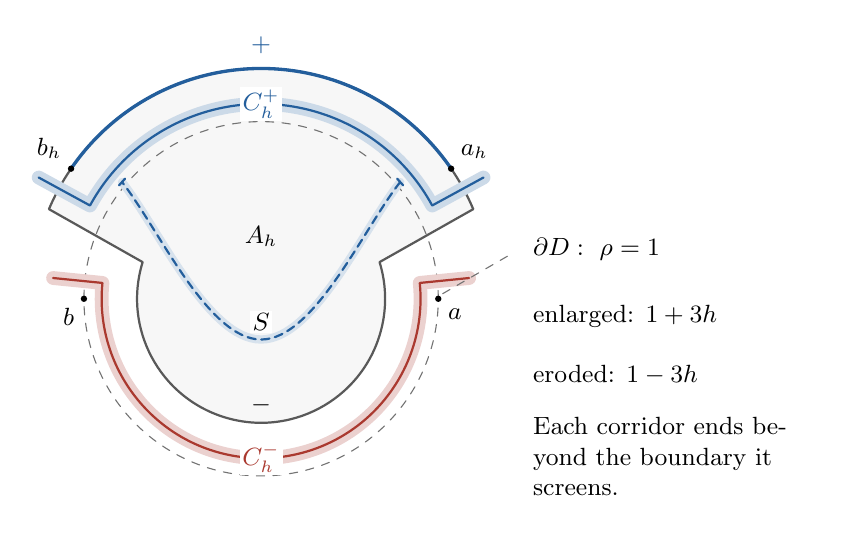
\begin{tikzpicture}[scale=2.25,line cap=round,line join=round,
  every node/.style={font=\small}]
 \definecolor{curveplus}{RGB}{35,94,156}
 \definecolor{curveminus}{RGB}{170,57,47}
 \fill[black!3]
   (17.2:.70)--(22.9:1.30) arc[start angle=22.9,end angle=157.1,radius=1.30]
   --(162.8:.70) arc[start angle=162.8,end angle=377.2,radius=.70]--cycle;
 \draw[black!65,thick]
   (17.2:.70)--(22.9:1.30) arc[start angle=22.9,end angle=157.1,radius=1.30]
   --(162.8:.70) arc[start angle=162.8,end angle=377.2,radius=.70];
 \draw[curveplus,very thick]
   (34.4:1.30) arc[start angle=34.4,end angle=145.6,radius=1.30];
 \draw[dashed,black!55] (0,0) circle[radius=1];
 \draw[curveminus!23,line width=5pt]
   (174.3:1.18)--(174.3:.90)
   arc[start angle=174.3,end angle=365.7,radius=.90]--(5.7:1.18);
 \draw[curveminus,thick]
   (174.3:1.18)--(174.3:.90)
   arc[start angle=174.3,end angle=365.7,radius=.90]--(5.7:1.18);
 \draw[curveplus!23,line width=5pt]
   (28.6:1.43)--(28.6:1.10)
   arc[start angle=28.6,end angle=151.4,radius=1.10]--(151.4:1.43);
 \draw[curveplus,thick]
   (28.6:1.43)--(28.6:1.10)
   arc[start angle=28.6,end angle=151.4,radius=1.10]--(151.4:1.43);
 \draw[curveplus!18,line width=3pt]
   (40:1.025) .. controls (.58,.40) and (.30,-.23) .. (0,-.23)
   .. controls (-.30,-.23) and (-.58,.40) .. (140:1.025);
 \draw[curveplus,densely dashed,thick]
   (40:1.025) .. controls (.58,.40) and (.30,-.23) .. (0,-.23)
   .. controls (-.30,-.23) and (-.58,.40) .. (140:1.025);
 \draw[curveplus,thick] (.768,.678)--(.802,.640);
 \draw[curveplus,thick] (-.768,.678)--(-.802,.640);
 \node[fill=white,inner sep=1pt] at (0,-.13) {$S$};
 \fill (0:1) circle[radius=.018] node[below right] {$a$};
 \fill (180:1) circle[radius=.018] node[below left] {$b$};
 \fill (34.4:1.30) circle[radius=.018] node[above right] {$a_h$};
 \fill (145.6:1.30) circle[radius=.018] node[above left] {$b_h$};
 \node at (0,.35) {$A_h$};
 \node[curveplus,fill=white,inner sep=1pt] at (0,1.10) {$C_h^+$};
 \node[curveminus,fill=white,inner sep=1pt] at (0,-.90) {$C_h^-$};
 \node at (0,-.60) {$-$};
 \node[curveplus] at (0,1.43) {$+$};
 \node[anchor=west] at (1.48,.28) {$\partial D:\ \rho=1$};
 \draw[dashed,black!55] (1.39,.24)--(1.01,.02);
 \node[anchor=west] at (1.48,-.10) {enlarged: $1+3h$};
 \node[anchor=west] at (1.48,-.43) {eroded: $1-3h$};
 \node[anchor=west,align=left,text width=3.7cm] at (1.48,-.89)
   {Each corridor ends beyond the boundary it screens.};
\end{tikzpicture}

 \caption{The minus-favoring construction for a small displacement $h>0$,
 in Schoenflies coordinates. Here $A_h$ is a sufficiently close polygonal
 approximation, in the physical plane, of the preliminary displaced
 topological domain; $a_h,b_h$ are its incoming and outgoing boundary marks.
 The dashed circle is $\partial D$. The preliminary boundary is enlarged
 along its middle plus arc and eroded elsewhere. The red minus corridor
 $C_h^-$ is outside $A_h$, including its caps; the blue plus corridor
 $C_h^+$ is outside $D$, and crosses the minus boundary of $A_h$ before
 its end gates. Corridor widths and radial displacements are exaggerated.
 The dashed blue strip $S$ illustrates an allowed plus strip: its gates
 lie just outside $D$, and the strip lies inside $A_h$, on the center
 side of both corridors.  Such strips are selected from a finite
 deterministic list before coupling any crossing events.  The diagram
 specifies topology and signs, not a metric distortion estimate for
 $\Psi$.}
 \label{fig:boundary-squeeze}
\end{figure}

Replace the boundary, corridors, scopes, and gates by sufficiently close
polygonal approximations in the physical plane.  One way to do this is
to subdivide each of the finitely many simple arcs into pieces lying in
disjoint small neighborhoods of nonadjacent pieces, then join points in
successive neighborhoods by polygonal arcs; small transverse polygonal
gates give the rectangles. The rectangular neighborhoods of the arcs
are transported from the coordinate plane by $\Psi$. Working within
these neighborhoods preserves the order and sides in the polygonal
approximations.  All the displayed disjointness conditions, cap
crossings, and gaps between designated arcs are open conditions with
positive clearance.  Hence they survive sufficiently close
approximations.  Denote the resulting polygonal domain by $A_h$ and its
marked points by $a_h,b_h$.  Choose the approximation errors tending to
zero with $h$, including in boundary parametrization.  Ordinary lattice
approximations of this fixed polygonal marked domain will always be used
for its pure Dobrushin law.

For the comparison favoring plus use the radial function
$R_h(\theta-\pi)$ instead.  Its incoming and outgoing marks have angles
$2\pi-6h$ and $\pi+6h$, respectively; the enlarged intervening arc
through $3\pi/2$ is minus, and its complement is plus.  Rotate the two
corridor placements by $\pi$ and interchange their colors.  Thus the
inner plus corridor lies outside this comparison domain and the outer
minus corridor lies outside $D$.  Orient its pure chord from the mark
near $a$ to the mark near $b$, as before.

We spell out why these are valid comparisons for the given target
approximations.  If $c$ parametrizes $\partial D$, then $\phi_n\circ c$
parametrizes $\partial D_n$ and converges uniformly to $c$.  On any compact
set disjoint from $\partial D$, winding numbers of these curves agree
eventually; thus membership in $D_n$ agrees there with membership in $D$.
On a closed subarc separated from $a,b$, the order along the boundary is
also preserved, since $\phi_n$ is a homeomorphism taking the two marks to
the prescribed marks.  Consequently every fixed clearance, inclusion,
and signed-arc placement above holds for $D_n$ for all sufficiently large
$n$.  Fine teeth or fjords lie in the shrinking boundary collar.  They do
not replace any actual exterior pin, and they do not intersect a compact
clearance chosen at fixed $h$.

An allowed \emph{plus strip} is a polygonal topological rectangle $S$
with two end gates, whose closure is in $A_h$, on the center side of both
cutting corridors and outside both reveal scopes.  Its two gates are
outside $\overline D$, on the enlarged plus portion.  We may require
$S\subset\Psi(\{\rho<1+h/2\})$, with a slight decrease of this bound
to absorb polygonal tolerances.  Wherever $S$ crosses $\partial D$, it
does so on $I_+$ with positive clearance from the marks.  Only strips
satisfying all these conditions are used.  The relevant portion of $A_h$
is on the center side of $C_h^-$ because that entire corridor is outside
$A_h$.  The strips needed below exist around compact subarcs of a pure
interface; their selection will be justified separately.

\begin{proposition}[Fixed-geometry boundary squeeze]
\label{prop:boundary-squeeze}
Fix the domain, signs, a displacement $h$, the preceding polygonal
placements, and a finite list $S_1,\ldots,S_m$ of allowed plus strips.
Let $V_A\in\{0,1\}^m$ record their plus crossings in the pure Dobrushin
law in an ordinary mesh approximation of $A_h$.  Let $V_n^+$ record plus
crossings in the target, filling the portions of the strips outside
$D_n$ virtually with plus.  There is a coupling with
\begin{equation}
 \P(V_A\leq V_n^+)=1-o(1) \qquad(n\longrightarrow\infty),
 \label{eq:curves-vector-order}
\end{equation}
where the inequality holds coordinatewise.  The error is uniform over
all admissible target exterior configurations.  The sign-reversed
construction gives the corresponding transfer of minus crossings from
pure domains favoring plus.  The smallness condition on $\lambda$ is the
one fixed at the beginning of the section; only the mesh threshold and
the error bound depend on these fixed geometries.
\end{proposition}

\begin{proof}
Place all sets in a torus chart with a fixed positive external buffer.
Let $E_h$ be the event of simultaneous lengthwise minus and plus
crossings of $C_h^-$ and $C_h^+$.  Proposition~\ref{prop:pure-rsw} gives
$\mu_{0,N}(E_h)\geq q_h>0$ for small mesh.  By
Theorem~\ref{thm:bulk-stability}, $\mu_{\lambda,N}(E_h)\geq q_h/2$
eventually, and the joint laws of
\[
 \bigl(\one_{E_h},V(S_1),\ldots,V(S_m)\bigr)
\]
in the pure and perturbed tori have total variation distance
$\varepsilon_n\to0$.  Here each $V(S_i)$ is an ordinary bulk crossing
test in the torus, without virtual filling.  For any two laws $p,q$ on
a finite space, an event $E$ with $p(E),q(E)\geq q_*>0$, and a random
vector $V$ on that space, subtraction of the two conditional fractions
gives
\begin{equation}
 \bigl\|p(V\in\cdot\mid E)-q(V\in\cdot\mid E)\bigr\|_{\TV}
 \leq \frac{2\|p-q\|_{\TV}}{q_*}.
 \label{eq:curves-conditioned-tv}
\end{equation}
Thus the two middle vectors conditioned on $E_h$ can be coupled to agree
with probability $1-o(1)$.  The laws $p,q$ in this application are the
joint indicator laws just displayed; no total variation estimate on the
underlying spin fields is used.

In each conditioned torus reveal the crossing closest to the radially
exterior side of each corridor.  Use the stopped reveal of
Lemma~\ref{lem:comparison-stopped-reveal}.  The transcript examines the
exterior side up to the crossing and leaves only pins of its prescribed
color facing the center.  The crossing and the event of its being the
first such crossing are determined by this transcript.  After both
transcripts have been conditioned upon, no additional crossing-existence
condition remains on the unrevealed center.  The two scopes are disjoint,
so the second reveal does not enter the core left by the first.

For precision, the free comparison components and all their boundary
incidences are as follows.  In the first comparison, the lower law is the
pure law in $A_h$, and the upper law is the conditioned pure torus.  Take
the components of the common free region on the center side of its
revealed plus path.  This path is an upper plus pin against lower free
spins.  All accessible portions of $\partial A_h$ are lower minus pins
against upper free spins: the plus boundary is screened by the revealed
path, whose caps continue outside $A_h$.  At a meeting of a path and a
boundary, the pair is upper plus against lower minus.  The minus reveal
is outside $A_h$ by~\eqref{eq:curves-scope-clearances}.  These checks give
a joint comparison on all spins used by the strips, and therefore
\[
 V_A\leq V_0^{E_h}.
\]

In the second comparison the lower law is the conditioned perturbed
torus and the upper law is the target.  Take the common free components
on the center side of the revealed minus path.  On this path the lower
pin is minus and the upper vertex is free.  The target minus arc is
screened by this path and its caps.  Every remaining accessible target
boundary neighbor is an upper plus pin against a lower free vertex.
Where the two cuts meet, the pair is upper plus against lower minus.
The plus reveal lies outside the target.  The comparisons are precisely
\[
 (\text{upper},\text{lower})=(+,\text{free}),\quad
 (\text{free},-),\quad (+,-).
\]
No same-sign pinned pair, and no monotonicity of an arbitrary pinned
perturbed factor, is being assumed.  A diagonal segment of a separating
triangulated path cannot be crossed by the interior of a nearest-neighbor
edge.  Thus each nearest-neighbor incidence leaving a comparison
component actually meets one of the path or arc pins just enumerated.
This remains true when a strip exits and reenters $D_n$.  Condition on
all other auxiliary bits as in Proposition~\ref{prop:strict-incidence};
the strict inequalities are uniform in those bits and hence in the
unprescribed spin pattern farther behind the arcs.  The resulting spin
comparison and the extremal virtual values outside $D_n$ give
\[
 V_\lambda^{E_h}\leq V_n^+.
\]

Finally glue the two order couplings with the equality coupling supplied
by~\eqref{eq:curves-conditioned-tv}.  This is elementary disintegration
on finite spaces: first sample each common middle vector, then sample
the remaining variables from the relevant conditional laws.  Extend the
outer vectors to their complete configurations in the same way.  This
proves~\eqref{eq:curves-vector-order}.  In particular the conclusion is
about a finite vector of tests, not a total variation comparison of spin
configurations.  Interchanging plus and minus and exchanging the
enlarged and eroded arcs proves the other assertion.
\end{proof}

The virtual filling in the proposition is a rule for evaluating a spin
crossing.  We now justify its use as a geometric barrier, including at
corners of the target boundary.

\begin{lemma}[Local drawing beside a signed strip]
\label{lem:curves-local-barrier}
Fix finitely many allowed plus strips and, in the sign-reversed
construction, finitely many allowed minus strips.  For all sufficiently
large $n$, the prescribed target curve has a drawing $\widetilde\gamma_n$
with the same traversal order and
\[
 d_{\rm curv}(\widetilde\gamma_n,\gamma_n)=O(\delta_n)
\]
that is disjoint from every monochromatic crossing of its respective
virtually filled strip.  The two half-stubs and neighborhoods of the
marks can retain their original drawings.  The filling and redrawing
change no spin in the conditional law and remove no interaction term.
\end{lemma}

\begin{proof}
Consider first a plus strip.  Its boundary contacts lie on a compact
subarc of $I_+$ separated from the marks.  For large $n$, the same is
true of its contacts with $\partial D_n$.  Every exterior vertex sharing
a nearest-neighbor bond with the domain at those contacts is already
plus, by Lemma~\ref{lem:contour-spin}.  Fill the remaining exterior
vertices of the incident square faces with plus for the purpose of
drawing only.

Inspect a square face of the primal lattice, or equivalently the four
cells incident to one dual vertex.  The Jordan condition allows one,
two adjacent, or three interior cells at a boundary vertex; two opposite
interior cells alone would give a diagonal pinch.  With one interior
cell, its two nearest exterior neighbors are already plus.  Only the
opposite exterior vertex might have a different actual spin, and filling
it leaves every disagreement edge in $E_{\Omega_n}$ unchanged.  The
resulting zero set joins the two occupied domain edges when there are
two.  With two adjacent or three interior cells, every exterior cell
of the face is a nearest exterior neighbor, so its spin already has the
filling value.  In each case the interpolated zero segments have exactly
the partial contour's connections: its unique connection at degree two,
and the prescribed NE/SW pairing at degree four.  Faces wholly inside
the domain have the same property without filling.

Redraw the target portions in all faces meeting the strip, together
with one adjacent lattice layer, as the corresponding zero segments.
A monochromatic edge of the triangulation is disjoint from that zero
set.  Both the original drawing and each replacement meet a face side
at the same disagreement-edge midpoint.  The replacements therefore
glue to one another and to the unchanged portions without changing a
local connection.  Matching the successive face crossings in their
original order gives the displayed $O(\delta_n)$ curve distance.

The minus construction is identical with the colors exchanged.  The
boundary-contact sets of the fixed plus and minus strip lists have
positive separation from each other and from the marks.  Therefore,
for sufficiently fine mesh, no face receives conflicting filling
instructions.  In the bulk both instructions use the actual spins.
The replacements can consequently be made simultaneously, leaving the
marked neighborhoods and half-stubs untouched.  This is a modification
of the drawing, not an interpolation of the actual full-plane exterior
configuration.  In particular all farther exterior spins and every
interaction across a narrow fjord remain in the Gibbs conditional law.
\end{proof}

\subsection{From fixed strip tests to limiting barriers}

We first record the domain-continuity fact needed for the displaced pure
curves.  If Jordan boundaries $c_j:\partial\mathbb D\to\partial G_j$
are homeomorphic parametrizations converging uniformly to a Jordan
parametrization $c$, normalized conformal maps
$f_j:\mathbb D\to G_j$ converge uniformly on $\overline{\mathbb D}$
to the corresponding map onto $G$.  Normalization can be by one fixed
interior point and positive derivative, or by three convergent distinct
boundary points.  Here is the reason the boundary assumption matters.
Uniform convergence to the injective $c$ implies a uniform local
connectedness modulus for the boundaries: nearby endpoints have one
boundary subarc of small diameter.  Indeed, otherwise inverse
uniform continuity of $c$ and uniform continuity of the parametrizations
would give two separated parameter arcs with arbitrarily close images.
Kernel convergence gives local uniform convergence of the normalized
maps.  The boundary crosscut proof of the Carath\'eodory extension
theorem, applied with this common local connectedness modulus, gives
equicontinuity on the closed disk, and hence upgrades local convergence
to uniform convergence.  This is Rad\'o's Jordan-domain continuity
theorem \citep[Th\'eor\`eme, p.~182]{Rado1923}.  Its stated uniform
convergence is on the closed disk.  It requires more than kernel
convergence alone.

For clarity, the crosscut argument is uniform here.  The image areas are
bounded by a common containing disk.  Cauchy--Schwarz on circular arcs
centered at a boundary point of $\mathbb D$, followed by integration in
their radii, supplies a crosscut of image length tending to zero between
any two sufficiently small separated radius scales; the squared length
bound is a constant divided by the logarithm of their ratio.  Its image
endpoints are close.  The common local connectedness modulus bounds the
diameter of the smaller boundary subarc joining them.  The image
crosscut together with that subarc cuts off a set of comparably small
diameter.  The component not containing the fixed normalized interior
point is this small component, since that point has fixed positive
distance from the boundary.  This controls the images of the smaller
boundary neighborhood uniformly.  Finite covering of the unit circle
then proves the required equicontinuity.  Boundary normalization follows
by precomposing with disk automorphisms; the preimages of the three
distinct limiting marks converge by injectivity of the limiting boundary
map.

To account explicitly for the moving marks, first normalize $f_h,f$ by
a common interior point and positive derivative.  If $\alpha_h,\beta_h$
are the boundary preimages of $a_h,b_h$, uniform convergence on the
closed disk and injectivity of $f$ imply
$\alpha_h\to\alpha=f^{-1}(a)$ and
$\beta_h\to\beta=f^{-1}(b)$.  Fix a third boundary point different
from $\alpha,\beta$.  The disk automorphism taking
$\alpha,\beta$ to $\alpha_h,\beta_h$ and fixing that third point
converges uniformly on the closed disk to the identity.  Precomposition
by these automorphisms therefore gives uniformly convergent maps with
the required marked endpoints.

Applying this fact to $A_h$, and coupling by a single disk $\SLE_3$,
shows that its continuum pure interface law converges as $h\downarrow0$
to chordal $\SLE_3$ in $D$ from $a$ to $b$, in the oriented uniform curve
metric.  The same holds for the plus-favoring comparison domains.  This
uses the conformal definition of $\SLE_3$ and its continuous simple trace;
uniform convergence of the conformal maps bounds the distance between
the corresponding image curves.  For fixed $h$ the lattice convergence
used here is only Theorem~\ref{thm:pure-sle} in an ordinary polygonal
approximation of $A_h$.

\paragraph{Choosing a deterministic finite list.}
Couple
the continuum curves in $A_h$ to their limit $\Gamma$ so that their
oriented distances tend to zero.  The curve $\Gamma$ meets $\partial D$
only at $a,b$.  For every fixed small parameter interval removed from
each end, its remaining compact subarc is a positive distance inside
$D$.  Uniform convergence implies that, with probability tending to one
as $h\downarrow0$, a middle subarc of the curve in $A_h$ lies below
$\rho=1+h/2$, has endpoints outside $\overline D$, and the omitted
terminal pieces have diameter tending to zero.  To make this choice
without a regularity assumption on level hits, choose a point of the
curve deep inside $D$, take the last hit of $\rho=1+h/3$ before that
point and the first hit after it.  The intervening subarc lies in
$\rho\leq1+h/3$.  Both hits lie outside $D$ on the enlarged plus arc.
Extend this subarc slightly at its two ends, within
$\rho<1+h/2$, before choosing gates.  Compact parts away from $a,b$
cannot contain these hits in the limit.  The omitted portions therefore
shrink in diameter.  Polygonal tolerances can be chosen smaller than the
gaps between these levels.

For each such simple subarc, a rectangular neighborhood of a slightly
extended arc gives a thin strip with transverse end gates lying outside
$D$.  Polygonal approximation of its sides and gates gives an allowed
strip.  One can prescribe a continuous parametrization of its
cross-sections such that each section has small diameter and stays near
the corresponding point of a simple polygonal prototype.  A lengthwise
traversal then stays near this prototype, even if it backtracks.  The
extended subarc crosses both gates with a margin, and stays away from
the long sides.  These properties persist in an open neighborhood in
the oriented curve metric.  On sufficiently fine lattices, a traversal
by the pure interface with these margins supplies a plus spin crossing
of the strip: follow its plus side in the fixed triangulation and crop
at the gates.  The discrepancy between that side and the interface is
$O(\delta_n)$, smaller than the fixed margin.

The strip construction can be made from a countable collection, using
rational polygonal vertices and rational positive margins.  These open
curve neighborhoods cover all the favorable continuum curves just
described.  The curve space is separable; equivalently use this explicit
countable collection and continuity from below of probability.  A finite
subcollection thus covers all but any prescribed positive probability.
Fix that entire finite list before using
Proposition~\ref{prop:boundary-squeeze}.  After its joint vector coupling
has been made, the pure curve may select one strip from the list.  The
corresponding target crossing then exists outside an event of vanishing
probability.  No test chosen adaptively from an infinite family has
been inserted into Theorem~\ref{thm:bulk-stability}.

\paragraph{Passing to moving geometries.}
Choose errors
$\epsilon_j\downarrow0$.  First choose $h_j\downarrow0$, polygonal
comparison domains of both signs, and favorable continuum events whose
omitted end pieces have diameter at most $\epsilon_j$, with failure
probability at most $\epsilon_j$.  Then choose finite strip covers with
widths and prototype errors at most $\epsilon_j$ and additional failure
probability at most $\epsilon_j$.  Finally choose increasing integers
$n_j$ so that for every $n\geq n_j$ the fixed placements, both pure
interface approximations, and both finite-vector couplings have all
their required errors at most $\epsilon_j$.  Set
\begin{equation}
 j(n)=\max\{j\leq n:n_j\leq n\},
 \label{eq:curves-slow-diagonal}
\end{equation}
with an arbitrary definition before $n_1$.  This index tends to infinity.
The constants $q_{h_j}$ in~\eqref{eq:curves-conditioned-tv} may tend to
zero; the threshold $n_j$ has already absorbed their reciprocals.
Couple each of the two comparison constructions with the target and
glue over the target configuration.  Their comparison curves need not
be independent.  Both marginal laws converge to the same chordal
$\SLE_3$ law, and, with probability tending to one, the target has both
colored barriers in strips converging to those comparison curves.

\subsection{Forbidden sides, order, and identification of the trace}

For a simple chord $C$ of $D$ from $a$ to $b$, with interior in $D$, let
$P(C)$ and $M(C)$ be the open components of $D\setminus C$ adjacent to
$I_+$ and $I_-$, respectively.  Their closures below are in $\overline D$.
All target traces lie in one fixed compact set for large $n$.  The space
of nonempty compact subsets of that set is compact in Hausdorff distance.
Consequently, along any mesh subsequence we can pass further to a joint
limit
\[
 (\operatorname{tr}\gamma_n,L_n,U_n)\ \Longrightarrow\ (K,L,U),
\]
where $L_n,U_n$ are the two comparison curves in the slow diagonal.
Their marginal curve laws are tight by the preceding construction.
The limit $K$ is connected and contains $a,b$: separation of a compact
limit into two sets at positive distance would separate every
sufficiently close connected approximant.  Also $K\subset\overline D$:
winding stability excludes every fixed compact set outside
$\overline D$ from $D_n$ eventually, and the drawing displacements
vanish.  The curves $L,U$ have the
chordal $\SLE_3$ marginal law.  Use a representation of this joint
convergence in which the compact and curve distances tend to zero
almost surely, and pass to a further subsequence so that barrier failures
also occur only finitely often.

We claim that the barriers imply
\begin{equation}
 K\subset\overline{M(L)}\cap\overline{P(U)}.
 \label{eq:curves-forbidden-sides}
\end{equation}
Choose once and for all $\rho_*>1$, independently of $h$ and $n$, and
restrict to $h$ with $1+h/2<\rho_*$.  Consider the plus barrier associated
with $L_n$.  Erase loops from a successful strip crossing and connect its
ends to the gate centers within exterior gate neighborhoods.  In
Schoenflies coordinates, close this path by radial segments from the gate
centers to $\rho=\rho_*$ and the plus-side circular arc between them.
For each fixed $h$ these added paths have positive clearance from
$\overline D$, so they lie outside $D_n$ for all sufficiently large $n$;
include this requirement in the choice of $n_j$.  Together these paths
form a closed barrier disjoint from the redrawn target
$\widetilde\gamma_n$ of Lemma~\ref{lem:curves-local-barrier}.  We use
this exact disjointness here; $O(\delta_n)$ closeness alone would not
preserve disjointness from a lattice barrier.  Both target marks are on
its zero-winding exterior side: their outward escape paths
lie beyond the ends of the extended plus arc and avoid the strip, whose
ends are inside the target plus arc and separated from the marks.  Thus
the entire redrawn target interface has zero winding relative to the
closed barrier.

On every compact subset of $P(L)$, the barrier has, for large $n$, the
same nonzero winding as $L$ closed around $I_+$ outside $D$.  To verify
this without controlling the traversal order of the target crossing,
use the rectangular chart of the strip.  Any path connecting its two end
gates is homotopic, relative to those gates, to its central prototype;
its loops can be removed inside the strip.  Its winding about a point
outside that strip is therefore the prototype's winding.  The widths
vanish, the prototypes converge in curve distance to $L$, and the
terminal errors shrink to $a,b$.  The gate centers therefore tend to
$a,b$, and their radial connectors tend to the endpoint radial segments.
On every compact subarc of $I_+$, the fixed-radius part of the closure
stays a positive distance beyond $\partial D$, while the connectors
remain away from that subarc.  The same winding conclusion consequently
holds on small neighborhoods of every point of $I_+$ other than $a,b$.
The redrawn target cannot enter these neighborhoods.  Its trace has
the same Hausdorff limit $K$ as the original target, by
Lemma~\ref{lem:curves-local-barrier}.  This excludes both $P(L)$ and
the open plus boundary arc from $K$, leaving
$K\subset\overline{M(L)}$.  The minus barrier proves
$K\subset\overline{P(U)}$.  The half-stubs remain near the marks and
therefore do not meet these fixed neighborhoods.

\begin{lemma}[Ordered chords with equal laws]
\label{lem:ordered-chords}
Let $L,U$ be random simple chords from $a$ to $b$ in a Jordan domain,
meeting its boundary only at their endpoints, and let $K$ be a random
compact connected subset of its closure containing $a,b$.  Suppose
\eqref{eq:curves-forbidden-sides} holds almost surely.  Then
$P(L)\subset P(U)$ almost surely.  If $L$ and $U$ have the same trace
law, then $L=U=K$ as compact sets almost surely.
\end{lemma}

\begin{proof}
Work in the closed disk using a fixed Schoenflies map.  If
$P(L)\cap M(U)$ were nonempty, connect a point of that intersection to
an interior point of $I_+$ through $P(L)$ and to an interior point of
$I_-$ through $M(U)$.  The two side domains are Jordan domains.  Small
endpoint arcs and interior polygonal paths, with loops removed, therefore
give a simple crosscut between these opposite boundary arcs, contained
in their union except for its two boundary endpoints.  This crosscut is
disjoint from $K$ by~\eqref{eq:curves-forbidden-sides}.  Its endpoints
alternate with $a,b$ around the circle, so it separates $a$ from $b$ in
the closed disk.  This contradicts connectedness of $K$.  Hence
$P(L)\cap M(U)=\varnothing$.  It follows that
$P(L)\subset P(U)\cup U$.  No interior point of $U$ can lie in the open
set $P(L)$: every neighborhood of such a point meets $M(U)$.  Thus
$P(L)\subset P(U)$.

Let $X,Y$ be the ordinary planar areas of the two plus sides after this
fixed disk map.  They are bounded random variables, $X\leq Y$, and their
distributions agree when the trace laws agree.  Thus $\E(Y-X)=0$ and
$X=Y$ almost surely.  Proper inclusion of these particular side domains
would give strictly different areas.  Indeed a point of
$P(U)\setminus P(L)$ either belongs to $M(L)$, or lies on $L$; in the
latter case its open neighborhood in $P(U)$ meets $M(L)$.  In either
case the difference contains a nonempty open subset of $M(L)$, of
positive area.  Consequently $P(L)=P(U)$ and their interior boundaries
give the same chord.  This reasoning does not require the chords to
have zero area.  Finally~\eqref{eq:curves-forbidden-sides} puts $K$
inside that chord.  The inverse of a simple parametrization sends $K$
to a connected subset of $[0,1]$ containing both endpoints, which is all
of $[0,1]$.
\end{proof}

The lemma identifies every subsequential target trace limit as chordal
$\SLE_3$.  We have also excluded a boundary segment from that trace.
We have not yet excluded repeated forward and backward travel in a
thin neighborhood of the same chord.  The next argument supplies that
last distinction.

\subsection{Interior passages and the orientation of the limit}

For a compact $F\Subset D$ and a fixed $R>0$ small enough that all
radius-$2R$ neighborhoods of $F$ lie in $D$, let $\mathcal B_n(F;r,R)$
be the event that the target contour has at least four passages across
an annulus with some center in $F$, inner radius $r$, and outer radius
$R$.  Passages count disjoint parameter intervals, with endpoint hits
allowed to coincide, as in Section~\ref{sec:stability}.  Square or round
annuli can be used, after fixed-factor changes of radii.  We claim
\begin{equation}
 \lim_{r\downarrow0}\limsup_{n\to\infty}
 \P\bigl(\mathcal B_n(F;r,R)\bigr)=0.
 \label{eq:curves-uniform-bottleneck}
\end{equation}
Cover the fixed $2R$-neighborhood by finitely many interior boxes with
fixed positive free buffers.  Proposition~\ref{prop:interior-density}
compares each of their target spin marginals pointwise with a torus
marginal, with a constant independent of $r,n,\tau_n$.  A grid of mesh
comparable to $r$ has $O_F(r^{-2})$ centers.  Four target passages about
any center in $F$ give four passages about a nearest grid center from
radius $Cr$ to radius $R/C$, by cropping the same paths at their hits.
At each grid center enlarge this to the event $F_4$ that \emph{any}
locally resolved contours supply four passages through that annulus.
This enlarged event is determined by the spins in the annulus and a
one-face margin.  Identifying the marked target component is not local,
but is unnecessary for this upper bound.  The bulk drawing comparison
absorbs its $O(\delta_n)$ displacement into the fixed radius crops.

For each fixed $r$ the enlarged events are finitely many fixed bulk
tests of Section~\ref{sec:stability}, and the density comparison applies
to them.  Theorem~\ref{thm:bulk-stability} and
Proposition~\ref{prop:pure-four-passages} bound their torus mesh upper
limits by $C_R(r/R)^{2+c}$ for some $c>0$ when $r/R$ is small.  A union
bound and the fixed density constants give an upper bound $C_{F,R}r^c$
after the mesh limit.  This proves~\eqref{eq:curves-uniform-bottleneck}.
The buffer in the density comparison was fixed before $r$ decreased;
there is no density constant at a shrinking buffer hidden in this bound.
The finite grid union also gives a measurable upper event for arbitrary
centers, so no measurable choice of a center is required below.

\begin{lemma}[Progress coordinates and the full curve metric]
\label{lem:curve-upgrade}
Let $\Gamma:[0,1]\to\overline D$ be continuous and injective, with
$\Gamma(0)=a$, $\Gamma(1)=b$, and $\Gamma((0,1))\subset D$.  Let
$g_n:[0,1]\to\C$ be continuous simple curves whose endpoints tend to
$a,b$ and whose traces tend in Hausdorff distance to $\Gamma([0,1])$.
There are continuous functions $u_n:[0,1]\to[0,1]$ with endpoint
values tending to $0,1$ such that
\begin{equation}
 e_n:=\sup_t|g_n(t)-\Gamma(u_n(t))|\longrightarrow0.
 \label{eq:curves-coordinate-error}
\end{equation}
Put $B_n=\sup_{s<t}(u_n(s)-u_n(t))$.  If $B_n\to0$, then
$d_{\rm curv}(g_n,\Gamma)\to0$.  Conversely, for every fixed $0<\eta<1$, a backward
drop $B_n\geq\eta$, with $n$ sufficiently large, forces six disjoint
passages from radius $r$ to one fixed radius $R_\eta>0$, for every
$e_n<r<R_\eta$, about a center on
$\Gamma([\eta/2,1-\eta/2])\Subset D$.

For random curves, suppose the trace and endpoint convergence hold in
probability in a coupling with such a random $\Gamma$, and suppose
\eqref{eq:curves-uniform-bottleneck} holds for every deterministic
compact interior $F$ and sufficiently small fixed $R$.  Then
$d_{\rm curv}(g_n,\Gamma)\to0$ in probability in that coupling.
\end{lemma}

\begin{proof}
The inverse coordinate $\Gamma^{-1}$ is continuous on the compact
trace.  Extend it continuously, with values in $[0,1]$, to a compact
ambient neighborhood and call the extension $p$.  Setting
$u_n=p\circ g_n$ gives~\eqref{eq:curves-coordinate-error} by uniform
continuity: a point close to $\Gamma(v)$ has $p$-value close to $v$,
and hence is close to $\Gamma(p(\cdot))$.  The endpoints have the
asserted coordinates.

Here is the matching when drops vanish.  The running maximum
\[
 m_n(t)=\max_{s\leq t}u_n(s)
\]
is continuous, nondecreasing, and satisfies
$0\leq m_n(t)-u_n(t)\leq B_n$.  Its endpoint values tend to $0,1$.
For all large $n$ let
\[
 v_n(t)=\frac{m_n(t)-m_n(0)}{m_n(1)-m_n(0)},\qquad
 h_n(t)=(1-\kappa_n)v_n(t)+\kappa_n t,
\]
where $0<\kappa_n\downarrow0$.  Then $h_n$ is an increasing
homeomorphism of $[0,1]$ and $\|h_n-u_n\|_\infty\to0$.  If
$\omega_\Gamma$ denotes the modulus of continuity of $\Gamma$, then
\[
 d_{\rm curv}(g_n,\Gamma)
 \leq e_n+\omega_\Gamma(\|h_n-u_n\|_\infty)\longrightarrow0.
\]
This uses exactly the allowed matching in~\eqref{eq:curve-metric},
with the identity on $g_n$ and $h_n$ on $\Gamma$.

For the converse, the continuous function $u_n(s)-u_n(t)$ attains its
maximum on $0\leq s\leq t\leq1$.  If $B_n\geq\eta>0$, a maximizing
pair has $s<t$ and $u_n(s)-u_n(t)\geq\eta$.  Set
$c_n=(u_n(s)+u_n(t))/2\in[\eta/2,1-\eta/2]$.  When the endpoint
coordinate errors are less than $\eta/4$, each of the intervals
$[0,s]$, $[s,t]$, and $[t,1]$ has endpoints on opposite sides of
$c_n$, at coordinate distance at least $\eta/4$.  Each therefore
contains a visit to $c_n$.  Injectivity and compactness imply
\[
 q_\eta=\min_{|v-w|\geq\eta/4}|\Gamma(v)-\Gamma(w)|>0,
 \qquad
 d_\eta=\dist(\Gamma([\eta/2,1-\eta/2]),\partial D)>0.
\]
Choose $R_\eta<\min(q_\eta,d_\eta)/4$.  Once $e_n<R_\eta$, the
four anchor points $g_n(0),g_n(s),g_n(t),g_n(1)$ are outside the
radius-$R_\eta$ disk about $\Gamma(c_n)$, whereas each of the three
level visits is within $e_n$ of its center.  In each time interval crop
the incoming and outgoing portions at the last outer and first inner
hits, and at the last inner and first outer hits.  For every
$e_n<r<R_\eta$ this supplies two annular passages.  The six parameter
interiors are disjoint, and simplicity gives disjoint spatial interiors.
They are thus six passages in the stated convention, and in particular
at least four.  Fixed-factor cropping gives the same assertion for
square annuli.

We give the measurability and order of limits for a random $\Gamma$.
Take a measurable continuous representative, for example the image of
a disk SLE representative in the coupling above.  We need not choose
a random extension $p$.  Write
$\Delta_n=d_H(\operatorname{tr}g_n,\operatorname{tr}\Gamma)$,
$z_n=2\Delta_n+1/n$, and define instead
\begin{equation}
 u_n(t)=
 \frac{\int_0^1 v\,(z_n-|g_n(t)-\Gamma(v)|)_+\,dv}
      {\int_0^1 (z_n-|g_n(t)-\Gamma(v)|)_+\,dv}.
 \label{eq:curves-measurable-coordinate}
\end{equation}
The denominator is positive since every $g_n(t)$ is within $\Delta_n$
of the trace, and continuity gives a parameter interval with positive
weight.  This coordinate is continuous in $t$ and jointly measurable.
Let
\[
 \iota_\Gamma(r)=\sup\{|v-w|:|\Gamma(v)-\Gamma(w)|\leq r\}.
\]
It tends to zero as $r\downarrow0$.  All parameters receiving positive
weight in~\eqref{eq:curves-measurable-coordinate} have diameter at most
$\iota_\Gamma(2z_n)$, and their weighted average lies between their
extreme values.  Consequently
\[
 e_n\leq z_n+
 \omega_\Gamma(\iota_\Gamma(2z_n))\longrightarrow0
\]
in probability; the endpoint coordinate errors also tend to zero.
These assertions follow first almost surely along any subsequence on
which $\Delta_n$ and the endpoint errors converge almost surely, and
hence hold in probability for the full sequence.

Fix $0<\eta<1$ and an exceptional probability $\zeta>0$.  Since
$q_\eta,d_\eta$ are strictly positive random variables, choose
deterministic $q,d>0$ such that
\[
 \P(q_\eta<q\ \text{or}\ d_\eta<d)<\zeta.
\]
The random centers then lie in the deterministic compact set
$F_d=\{z\in\overline D:\dist(z,\partial D)\geq d\}$, and one
deterministic $R<\min(q,d)/8$ works.  For each fixed $0<r<R$,
the preceding six-passage argument, outside an event of probability
$\zeta+o(1)$, bounds the probability of a drop of size $\eta$ by
$\P(\mathcal B_n(F_d;r,R))$.  First let $n\to\infty$, then
$r\downarrow0$ using~\eqref{eq:curves-uniform-bottleneck}, and finally
$\zeta\downarrow0$.  Thus $B_n\to0$ in probability.  To deduce curve
distance convergence, first choose a deterministic coordinate tolerance
on which $\omega_\Gamma$ is small outside probability $\zeta$, then use
the running-maximum bound and let $n\to\infty$.  Finally remove
$\zeta$.  This localizes the continuity modulus as well as the
injectivity and boundary-distance moduli.  All annulus radii and compact
charts are deterministic before the mesh limit is taken.
\end{proof}

The simplicity used in this lemma holds for the prescribed locally
resolved interface: the resolved embedded graph has degree two except
at its two degree-one stub midpoints, so its connecting component is an
embedded arc.  Distinct visits to a small disk along that arc count as
distinct passages.  No estimate for path length is required.  The lemma
also explains why a separate boundary passage estimate is unnecessary
at this stage: the limiting chord avoids the boundary away from its
endpoints, and its short terminal parameter intervals have arbitrarily
small diameter by continuity.

\subsection{Completion of the universality theorem}

\begin{proof}[Proof of Theorem~\ref{thm:main}]
For the fixed finite-range real potential $U$, Lemma~\ref{lem:contour-spin}
converts the exact contour weight into a finite-range, even,
square-symmetric spin perturbation, with all interactions meeting the
interior retained.  Theorem~\ref{thm:transfer} and
Theorem~\ref{thm:critical-trajectory} give an analytic bulk choice
$\beta_c(J,U,\lambda)$ near
$\beta_0=\log(1+\sqrt2)/(2J)$, positive for sufficiently small real
$\lambda$ of either sign and equal to $\beta_0$ at zero.  Shrink this
interval once to satisfy the independent-edit stability threshold and
the finite-table strict-incidence margins.  This gives a number
$\lambda_0(J,U)>0$ before any choice of $D,a,b$, approximation, exterior
contours, corridor, or strip.  The universal fixed-shape bootstrap in
Theorem~\ref{thm:bulk-stability} is what permits all later fixed
geometries to use this same interval.

Fix any $|\lambda|<\lambda_0$, any bounded Jordan marked domain, any
sequence of meshes and uniformly boundary-parametrized Jordan lattice
domains in the theorem, and any admissible sequence $P_{o,n}$.  On each
subsequence pass further so that the choice of plus boundary arc is
fixed.  The exact conditional-law reduction permits the target to be
placed in a buffered torus chart while retaining all its exterior pins.
Finite range permits any continuation beyond that chart without changing
the conditional law.  Proposition~\ref{prop:boundary-squeeze}, the
finite strip construction, and the slow diagonal produce a joint limit
of every further Hausdorff-convergent subsequence with two comparison
chords of the same $\SLE_3$ law.  Their forbidden-side inclusions and
Lemma~\ref{lem:ordered-chords} identify the target trace with that chord.
Thus the target traces converge in law in Hausdorff distance to chordal
$\SLE_3$.

Lift the subsequential trace coupling to the target paths using their
conditional distributions given their traces.  At each mesh the spin
space is finite, so this disintegration is immediate and preserves every
target passage probability.  No tightness of these path variables is
needed to perform the lift.  The limiting chord already has a measurable
continuous representative from its SLE marginal.  The interior density
comparison and bulk
four-passage estimate give~\eqref{eq:curves-uniform-bottleneck}, uniformly
in the permitted exterior configurations.  Lemma~\ref{lem:curve-upgrade}
therefore gives convergence in probability in the oriented curve metric
in this representation, and hence convergence in distribution in that
metric.  Since every subsequence has a further subsequence with this
same limit, the full sequence converges.  This argument also gives
tightness in the requested curve topology; it did not assume it for
the perturbed paths.

\widowpenalty=10000
The conclusion concerns the prescribed $\gamma_n$.  The local
redrawings used for its barriers preserve traversal order and have
$O(\delta_n)$ curve distance from it; they were used only to identify
its trace limit.  The half-stubs remained part of the original curve,
with endpoints tending to $a,b$, and the orientation is always from
the incoming midpoint to the outgoing midpoint.  The unit-lattice
potential $U$ was fixed throughout; only coordinates were multiplied by
$\delta_n$.  No sign
condition on $U$ or $\lambda$, boundary regularity beyond the stipulated
Jordan parametrizations, or restriction on the additional exterior
contours was imposed.  The value of $\beta_c$ and its interval of
validity are consequently independent of every domain and boundary
choice required in the theorem.
\end{proof}
